\documentclass[10pt,a4paper]{article}
\usepackage{fontspec}
\setmainfont{Latin Modern Roman}
\usepackage{microtype}
\usepackage[margin=2.2cm]{geometry}
\usepackage{amsmath,amssymb}
\usepackage{graphicx}
\usepackage{booktabs,array}
\usepackage[hidelinks,pdfauthor={Sandhya Nossin},pdftitle={A one-parameter dark-energy law and a parameter-free bet for final DESI and Euclid},pdfcreator={},pdfproducer={}]{hyperref}
\newcolumntype{L}[1]{>{\raggedright\arraybackslash}p{#1}}
\setlength{\parskip}{0.3em}
\setlength{\parindent}{0pt}

\title{\vspace{-1.2cm}\textbf{A one-parameter dark-energy law and a parameter-free bet:\\ $\Omega_m = 0.3123$ for final DESI and Euclid}}
\author{Sandhya Nossin\\\small independent author, \href{mailto:sandhya.nos@proton.me}{sandhya.nos@proton.me}}
\date{\small 14 November 2026 · companion note to \emph{La gravité comme mesure générative}, v5.3, \href{https://doi.org/10.5281/zenodo.23422750}{doi:10.5281/zenodo.23422750}}

\begin{document}
\maketitle
\vspace{-0.6cm}

\begin{abstract}
\noindent I propose a phenomenological dark-energy law, S3-L, in which the dark-energy density is built from inscriptions of the Hubble horizon that dilute as $1/a$. It has a single constant, $\mu_0$, which replaces $\Omega_\Lambda$: for the expansion history it has as many parameters as $\Lambda$CDM. Fitted to DESI DR2 and Planck, $\mu_0 = 1.305 \pm 0.016$, with a weak preference over $\Lambda$CDM after a penalty for the laws tried. I also state a sharper, parameter-free bet, $\mu_0 = 4/3$, which imposes $\Omega_m = 0.3123$ and a specific shape of $D_M/D_H$; it is compatible with current data (about $1.4\sigma$) and will be judged by final DESI and Euclid from 2027. Main weak point: $S_8$. All tests were pre-registered; a one-minute script reproduces the background.
\end{abstract}

\noindent\fbox{\parbox{\dimexpr\textwidth-2\fboxsep-2\fboxrule}{\small I am not a physicist. The calculations were done with the help of an AI assistant (Claude, Anthropic), which is not a co-author, and were checked by other instances of the same AI, which is not an independent review. I would be grateful for any criticism, including a quick refutation.}}

\section{The law}
A fraction $f$ of the Hubble horizon is taken to be ``inscribed'' at each epoch,
\begin{equation}\label{eq:f}
  f = 1 - \exp\!\left[-\mu_0\,(H_0/H)^3\right].
\end{equation}
Each inscription is given a weight $T\ln 2$ at the horizon temperature $T = H/2\pi$ (a posited normalization), which then dilutes as $1/a$. This gives
\begin{equation}\label{eq:rho}
  \rho_{\rm DE}(a) \propto \frac{H^3}{a}\int_0^{a} a'H'\,\mathrm{d}\!\left(\frac{f}{H'^2}\right), \qquad
  E^2 = \Omega_m a^{-3} + \Omega_r a^{-4} + \rho_{\rm DE}/\rho_{\rm crit,0}.
\end{equation}
There is no free amplitude: $\mu_0$ fixes the dark-energy curve and flatness then fixes $\Omega_m$, so $\mu_0$ replaces $\Omega_\Lambda$ rather than adding to it. Today $f_0 = 0.729$ and $\Omega_{\rm DE} = 0.682$. The equation of state is $w(0) \approx -0.82$, crosses $-1$ once near $z \approx 0.43$, and is below $-1$ before; the acceleration weakens but never stops. Fitted as DESI would, through the CPL model that best reproduces the predicted distances, the law gives $(w_0, w_a) \approx (-0.70, -1.05)$, close to Linder's ``mirage'' line~\cite{linder07}; the position alone does not separate S3-L from mirage models, the full shape of $w(z)$ does.

\textbf{Status.} The three ingredients (a count in the Hubble volume, hence the exponent 3; ``each event takes a share of what remains'', hence the exponential; the $1/a$ dilution) are posited, not derived, and the law was formulated after seeing the DESI data. Left free, the exponent is $2.85^{+0.20}_{-0.18}$: 1 and 2 are excluded, 4 strongly disfavoured.

\section{Confronting current data}
\begin{center}\small
\begin{tabular}{@{}L{0.42\textwidth}L{0.52\textwidth}@{}}
\toprule
Comparison & Result \\
\midrule
S3-L vs $\Lambda$CDM, full CMB spectrum (CAMB) + DESI DR2~\cite{desi25} + Planck~\cite{planck18} & $\Delta\chi^2 = -5.2$ (no SNe), $-9.2$ (Dovekie SNe~\cite{dovekie}), before penalty; $w_0w_a$ (two more parameters): $-6.6$ \\
Penalty for $\approx 25$ laws tried ($2\ln N \approx 6.4$) & Dovekie: $-9.2 \to \approx -2.8$, below $2\sigma$; with Pantheon+~\cite{pantheonplus} the corrected evidence leans towards $\Lambda$CDM \\
$S_8$ (frozen prediction) & $0.850$; DES Y6~\cite{desy6} measures $0.789 \pm 0.012$, already below the refutation threshold $0.798$ set in advance \\
$H_0$ & $\approx 67.2$ km/s/Mpc: S3-L slightly worsens the tension with SH0ES ($5.5\sigma$ vs $4.4\sigma$) \\
\bottomrule
\end{tabular}
\end{center}
The supernova advantage comes entirely from the match between the nearby ($z<0.1$) and distant samples; above $z = 0.1$ alone $\Lambda$CDM does better~\cite{efstathiou24}. This is a weak preference, not a confirmation.

\section{The bet $\mu_0 = 4/3$}
In the interpretive framework of the essay, the inscribed cells are counted with the convention ``one cell = one Planck area, one unit of information per four cells'', and an event is a Planck cell extended over a fixed depth $R_*$. This gives $\mu_0 = (4/3)(R_H/R_*)^3$. \emph{The bet}: our horizon reaches that depth today, $R_* = R_H$, so $\mu_0 = 4/3$ exactly (the fitted value corresponds to $R_*/R_H = 1.007 \pm 0.004$).

With $\mu_0 = 4/3$, S3-L has \emph{no free parameter} for the dark-energy curve and imposes
\[
  \Omega_m = 0.3123 \quad(\text{almost independent of } h),\qquad H_0 = 67.46,\qquad \omega_c \approx 0.119 .
\]
In the full chain (CMB spectrum, DESI DR2) it costs $\Delta\chi^2 = +2.1$ against free S3-L ($+1.8$ with Dovekie), about $1.4\sigma$: compatible. Its $D_M/D_H$ departs from the best-fit $\Lambda$CDM of the same chain by $+1.1\,\%$ at $z = 0.30$, $-0.8\,\%$ at $0.93$ and $-1.47\,\%$ at $z \approx 1.5$ (fig.~\ref{fig}).

\textbf{Caveats.} The choice is not blind: $4/3$ was known to be close to $1.305$ before the convention was fixed. Another convention would give another value ($\mu_0 = 1$ is excluded). The bet fixes the number, not why the coincidence $R_* = R_H$ happens in our epoch.

\begin{figure}[h]
\centering
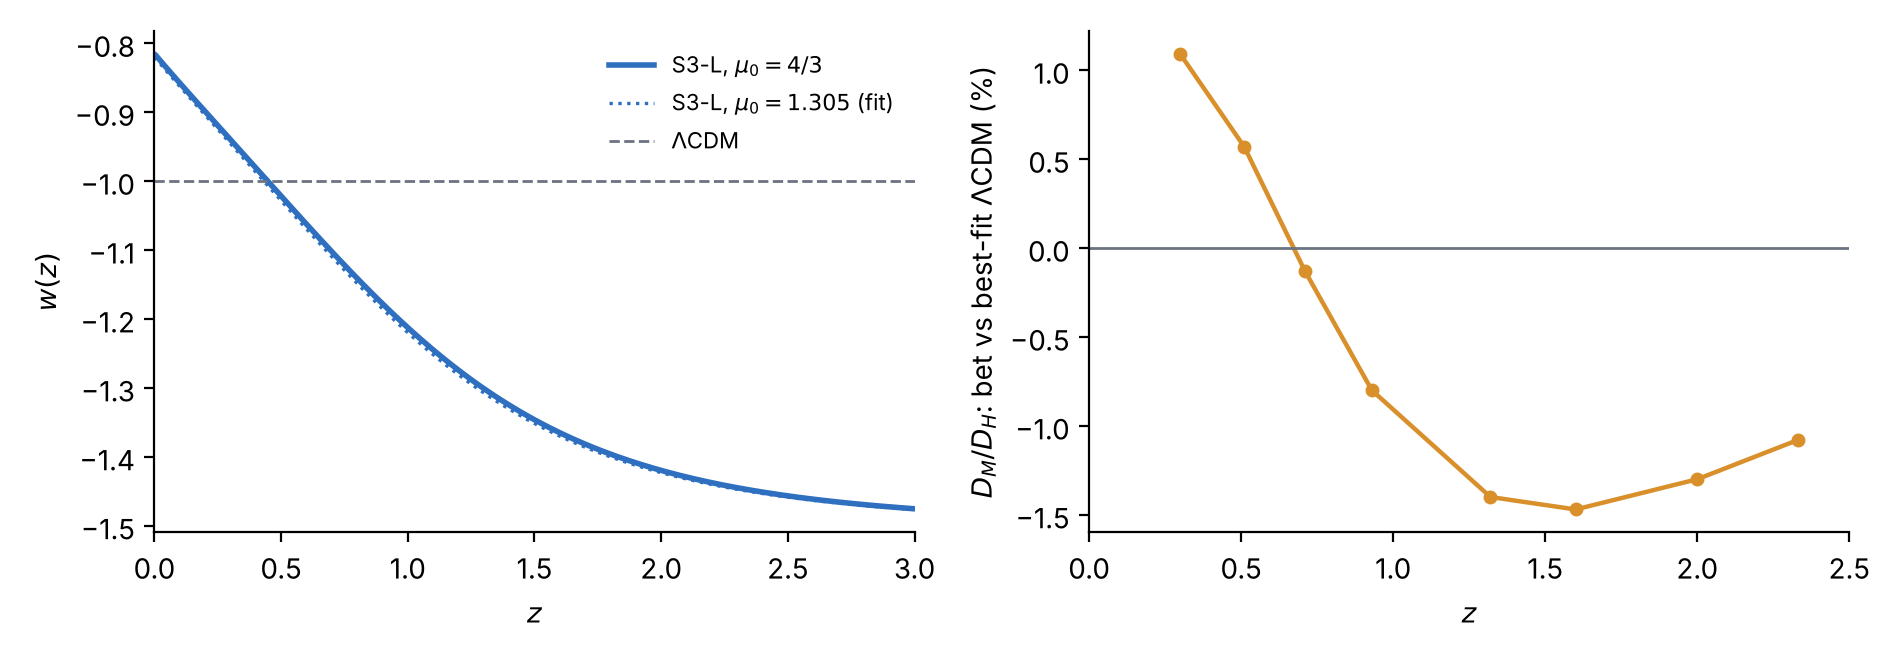
\includegraphics[width=0.96\textwidth]{fig_bet.png}
\caption{Left: $w(z)$ for the bet $\mu_0 = 4/3$ and for the fitted value. Right: $D_M/D_H$ of the bet relative to the best-fit $\Lambda$CDM of the same full chain (test no.~423).}\label{fig}
\end{figure}

\section{What would refute it}
\begin{center}\small
\begin{tabular}{@{}L{0.40\textwidth}L{0.17\textwidth}L{0.37\textwidth}@{}}
\toprule
Prediction & Data & Refuted if \\
\midrule
Bet: $\Omega_m = 0.3123$, $D_M/D_H$ within $1.5\,\%$ of $\Lambda$CDM, largest deviation near $z \approx 1.5$ & final DESI, Euclid (2027) & $\Omega_m$ incompatible with $0.3123$ at $>3\sigma$ (the bet falls; S3-L with fitted $\mu_0$ remains) \\
S3-L vs $\Lambda$CDM: expected separation $\approx 4.8\sigma$ (DESI alone $2.4$--$2.8\sigma$) & Euclid DR1 + final DESI & $\chi^2(\text{S3-L}) - \chi^2(\Lambda\text{CDM}) \ge +9$, or $(w_0,w_a)$ excluding the S3-L curve at $3\sigma$ \\
$S_8 = 0.850$ (frozen) & Euclid DR1 (mid-2027) & $S_8 < 0.798$ \\
\bottomrule
\end{tabular}
\end{center}
The refutation criteria were frozen before any Euclid data (4 November 2026); the bet line was added on 13 November 2026, knowing current data, and is declared as such.

\section{Reproducibility and method}
A self-contained script (\texttt{s3l\_check.py}, numpy and scipy) solves eq.~\eqref{eq:rho} and reproduces $\Omega_m = 0.3123$ for $\mu_0 = 4/3$ in about a second. The full fits (CAMB, DESI DR2, four supernova catalogues) and the code are in the Zenodo archive. Every test of the essay (numbered 1 to 440) was pre-registered: expected results written and fingerprinted (sha256, freeze time) before the code ran; failures are published in a separate document. The broader essay also contains an interpretive part (postulates on gravity, the Higgs and dark matter) that motivated the law; it is not needed to test it.

\small
\begin{thebibliography}{9}\setlength{\itemsep}{0pt}
\bibitem{desi25} DESI Collaboration, ``DESI DR2 results II: Measurements of baryon acoustic oscillations and cosmological constraints'', \emph{Phys. Rev. D} \textbf{112}, 083515 (2025), arXiv:2503.14738.
\bibitem{planck18} Planck Collaboration, ``Planck 2018 results. VI. Cosmological parameters'', \emph{Astron. Astrophys.} \textbf{641}, A6 (2020).
\bibitem{dovekie} B.~Popovic et al., ``The Dark Energy Survey Supernova Program: a reanalysis of cosmology results and evidence for evolving dark energy with an updated type Ia supernova calibration'', arXiv:2511.07517 (2025).
\bibitem{pantheonplus} D.~Brout et al., ``The Pantheon+ analysis: cosmological constraints'', \emph{Astrophys. J.} \textbf{938}, 110 (2022).
\bibitem{desy6} T.~M.~C.~Abbott et al. (DES), ``Dark Energy Survey Year 6 Results: Cosmological Constraints from Galaxy Clustering and Weak Lensing'', arXiv:2601.14559 (2026).
\bibitem{efstathiou24} G.~Efstathiou, arXiv:2408.07175 (2024).
\bibitem{linder07} E.~V.~Linder, ``The mirage of $w = -1$'', arXiv:0708.0024 (2007).
\end{thebibliography}
\end{document}
